%%%%%%%%%%%%%%%%%%%%%%%%%%%%%%%%%%%%%%%%%%%%%%%%%%%%%%%%%%%%%%%%%%%%%%%%%%%%%%%%%%%%%%%%%%%%%%%%%%%%%%%%%%%%%%%%%%%%%%%%%%%%%%%%%%%%%%%%%%%%%%%%%%%%%%%%%%%
% This is just an example/guide for you to refer to when submitting manuscripts to Frontiers, it is not mandatory to use frontiers.cls nor frontiers.tex  %
% This will only generate the Manuscript, the final article will be typeset by Frontier after acceptance.                                                 %
%                                                                                                                                                         %
% When submitting your files, remember to upload this *tex file, the pdf generated with it, the *bib file (if bibliography is not within the *tex) and all the figures.
%%%%%%%%%%%%%%%%%%%%%%%%%%%%%%%%%%%%%%%%%%%%%%%%%%%%%%%%%%%%%%%%%%%%%%%%%%%%%%%%%%%%%%%%%%%%%%%%%%%%%%%%%%%%%%%%%%%%%%%%%%%%%%%%%%%%%%%%%%%%%%%%%%%%%%%%%%%

%%% Version 3.0 Generated 2014/12/19 %%%
%%% You will need to have the following packages installed: datetime, fmtcount, etoolbox, fcprefix, which are normally inlcuded in WinEdt. %%%
%%% In http://www.ctan.org/ you can find the packages and how to install them, if necessary. %%%

\documentclass{frontiersSCNS} % for Science, Engineering and Humanities and Social Sciences articles
%\documentclass{frontiersHLTH} % for Health articles
%\documentclass{frontiersFPHY} % for Physics articles

%\setcitestyle{square}
\usepackage{url,lineno}
\linenumbers


% BELOW TAKEN FROM rticles plos template
%
% amsmath package, useful for mathematical formulas
\usepackage{amsmath}
% amssymb package, useful for mathematical symbols
\usepackage{amssymb}

% hyperref package, useful for hyperlinks
\usepackage{hyperref}

% graphicx package, useful for including eps and pdf graphics
% include graphics with the command \includegraphics
\usepackage{graphicx}

% Sweave(-like)
\usepackage{fancyvrb}
\DefineVerbatimEnvironment{Sinput}{Verbatim}{fontshape=sl}
\DefineVerbatimEnvironment{Soutput}{Verbatim}{}
\DefineVerbatimEnvironment{Scode}{Verbatim}{fontshape=sl}
\newenvironment{Schunk}{}{}
\DefineVerbatimEnvironment{Code}{Verbatim}{}
\DefineVerbatimEnvironment{CodeInput}{Verbatim}{fontshape=sl}
\DefineVerbatimEnvironment{CodeOutput}{Verbatim}{}
\newenvironment{CodeChunk}{}{}

% cite package, to clean up citations in the main text. Do not remove.
\usepackage{cite}

\usepackage{color}

% Below is from frontiers
%
\bibliographystyle{frontiersinSCNS}
% Use doublespacing - comment out for single spacing
%\usepackage{setspace}
%\doublespacing


% Leave a blank line between paragraphs instead of using \\



\def\keyFont{\fontsize{8}{11}\helveticabold }

%% ** EDIT HERE **
%% PLEASE INCLUDE ALL MACROS BELOW

%% END MACROS SECTION



 \def\Authors{
  Zhian N. Kamvar\,\textsuperscript{1},
  Jonah C. Brooks\,\textsuperscript{2},
  Niklaus J. Gr\"{u}nwald\,\textsuperscript{1,3*}}
% \\
\def\Address{
  \textsuperscript{1} Botany and Plant Pathology, Oregon State University,  Corvallis,  OR,  USA\\
  \textsuperscript{2} College of Electrical Engineering and Computer Science, Oregon State University,  Corvallis,  OR,  USA\\
  \textsuperscript{3} Horticultural Crops Research Laboratory, USDA-Agricultural Research Service,  Corvallis,  OR,  USA\\
}

  
  \def\firstAuthorLast{Kamvar {et~al.}}
  
  
  \def\corrAuthor{Niklaus J. Gr\"{u}nwald}\def\corrAddress{Horticultural Crops Research Laboratory USDA ARS\\3420 NW Orchard Ave.\\Corvallis, OR, 97330}\def\corrEmail{\href{mailto:grunwaln@science.oregonstate.edu}{\nolinkurl{grunwaln@science.oregonstate.edu}}}
  
%DIF PREAMBLE EXTENSION ADDED BY LATEXDIFF
%DIF UNDERLINE PREAMBLE %DIF PREAMBLE
\RequirePackage[normalem]{ulem} %DIF PREAMBLE
\RequirePackage{color}\definecolor{RED}{rgb}{1,0,0}\definecolor{BLUE}{rgb}{0,0,1} %DIF PREAMBLE
\providecommand{\DIFaddtex}[1]{{\protect\color{blue}\uwave{#1}}} %DIF PREAMBLE
\providecommand{\DIFdeltex}[1]{{\protect\color{red}\sout{#1}}}                      %DIF PREAMBLE
%DIF SAFE PREAMBLE %DIF PREAMBLE
\providecommand{\DIFaddbegin}{} %DIF PREAMBLE
\providecommand{\DIFaddend}{} %DIF PREAMBLE
\providecommand{\DIFdelbegin}{} %DIF PREAMBLE
\providecommand{\DIFdelend}{} %DIF PREAMBLE
%DIF FLOATSAFE PREAMBLE %DIF PREAMBLE
\providecommand{\DIFaddFL}[1]{\DIFadd{#1}} %DIF PREAMBLE
\providecommand{\DIFdelFL}[1]{\DIFdel{#1}} %DIF PREAMBLE
\providecommand{\DIFaddbeginFL}{} %DIF PREAMBLE
\providecommand{\DIFaddendFL}{} %DIF PREAMBLE
\providecommand{\DIFdelbeginFL}{} %DIF PREAMBLE
\providecommand{\DIFdelendFL}{} %DIF PREAMBLE
%DIF END PREAMBLE EXTENSION ADDED BY LATEXDIFF
%DIF PREAMBLE EXTENSION ADDED BY LATEXDIFF
%DIF HYPERREF PREAMBLE %DIF PREAMBLE
\providecommand{\DIFadd}[1]{\texorpdfstring{\DIFaddtex{#1}}{#1}} %DIF PREAMBLE
\providecommand{\DIFdel}[1]{\texorpdfstring{\DIFdeltex{#1}}{}} %DIF PREAMBLE
%DIF END PREAMBLE EXTENSION ADDED BY LATEXDIFF

\begin{document}
% \inputencoding{utf8}
\onecolumn
\firstpage{1}

\title[Novel R tools for population genomics]{Novel R tools for analysis of genome-wide population genetic data with
emphasis on clonality}
\author[\firstAuthorLast]{\Authors}
\address{}
\correspondance{}
\extraAuth{}% If there are more than 1 corresponding author, comment this line and uncomment the next one.
%\extraAuth{corresponding Author2 \\ Laboratory X2, Institute X2, Department X2, Organization X2, Street X2, City X2 , State XX2 (only USA, Canada and Australia), Zip Code2, X2 Country X2, email2@uni2.edu}
\topic{}% If your article is part of a Research Topic, please indicate here which.
\maketitle

\begin{abstract}

To gain a detailed understanding of how plant microbes evolve and adapt to
hosts, pesticides, and other factors, knowledge of the population dynamics and
evolutionary history of populations is crucial. Plant pathogen populations are
often clonal or partially clonal which requires different analytical tools. With
the advent of high throughput sequencing technologies, obtaining genome-wide
population genetic data has become easier than ever before. We previously
contributed the R package \textit{poppr} specifically addressing issues with
analysis of clonal populations. In this paper we provide several significant
extensions to \textit{poppr} with a focus on large, genome-wide SNP data.
Specifically, we provide several new functionalities including the new function
\texttt{mlg.filter} to define clone boundaries allowing for inspection and
definition of what is a clonal lineage, minimum spanning networks with
reticulation, a sliding-window analysis of the index of association, modular
bootstrapping of any genetic distance, and analyses across any level of
hierarchies.

\tiny
 \keyFont{ \section{Keywords:} clonality, population genomics, bootstrap, index of association, hierarchical analysis, sliding window}
\end{abstract}

\section*{Introduction}\label{introduction}
\addcontentsline{toc}{section}{Introduction}

To paraphrase Dobzhansky, nothing in the field of plant-microbe
interactions makes sense except in the light of population genetics
(Dobzhansky, 1973). Genetic forces such as selection and drift act on
alleles in a population. Thus, a true understanding of how plant
pathogens emerge, evolve and adapt to crops, fungicides, or other
factors, can only be elucidated in the context of population level
phenomena given the demographic history of populations (McDonald and
Linde, 2002; Gr\"{u}nwald and Goss, 2011; Milgroom et al., 1989). The field
of population genetics, in the era of whole genome resequencing,
provides unprecedented power to describe the evolutionary history and
population processes that drive coevolution between pathogens and hosts.
This powerful field thus critically enables effective deployment of R
genes, design of pathogen informed plant resistance breeding programs,
and implementation of fungicide rotations that minimize emergence of
resistance.

Most computational tools for population genetics are based on concepts
developed for sexual model organisms. Populations that reproduce
clonally or are polyploid are thus difficult to characterize using
classical population genetic tools because theoretical assumptions
underlying the theory are violated. Yet, many plant pathogen populations
are at least partially clonal if not completely clonal (Milgroom, 1996;
Anderson and Kohn, 1995). Thus, development of tools for analysis of
clonal or polyploid populations is needed.

Genotyping by sequencing and whole genome resequencing provide the
unprecedented ability to identify thousands of single nucleotide
polymorphisms (SNPs) in populations (Elshire et al., 2011; Luikart et
al., 2003; Davey et al., 2011). With traditional marker data (e.g., SSR,
AFLP) a clone was typically defined as a unique multilocus genotype
(MLG) (Gr{\"{u}}nwald and Hoheisel, 2006; Falush et al., 2003; Goss et al.,
2009; Cooke et al., 2012; Taylor and Fisher, 2003). Availability of
large SNP data sets provides new challenges for data analysis. These
data are based on reduced representation libraries and high throughput
sequencing with moderate sequencing depth which invariably results in
substantial missing data, error in SNP calling due to sequencing error,
lack of read depth or other sources of spurious allele calls
(Mastretta-Yanes et al., 2015). It is thus not clear what a clone is in
large SNP data sets and novel tools are required for definition of clone
boundaries.

The research community using the R statistical and computing language (R
Core Team, 2015) has developed a plethora of new resources for
population genetic analysis. R is particularly appealing because all
code is open source and functions can be evaluated and modified by any
user. Recently, we introduced the R package \emph{poppr} specifically
developed for analysis of clonal populations (Kamvar et al., 2014b).
\emph{Poppr} previously introduced several novel features including the
ability to conduct a hierarchical analysis across unlimited hierarchies,
test for linkage association, graph minimum spanning networks or provide
bootstrap support for Bruvo's distance in resulting trees. \emph{Poppr}
has been rapidly adopted and applied to a range of studies including for
example horizontal transmission in leukemia of clams (Metzger et al.,
2015), study of the vector-mediated parent-to-offspring transmission in
an avian malaria-like parasite (Chakarov et al., 2015), and
characterization of the emergence of the invasive forest pathogen
\emph{Hymenoscyphus pseudoalbidus} (Gross et al., 2014). It has also
been used to implement real-time, online R based tools for visualizing
relationships among unknown MLGs in reference
databases\\(\url{http://phytophthora-id.org/}) (Gr{\"{u}}nwald et al.,
2011).

Here, we introduce \emph{poppr} 2.0, which provides a major update to
\emph{poppr} (Kamvar et al., 2014b) including novel tools for analysis
of clonal populations specifically addressing large SNP data.
Significant novel tools include functions for calculating clone
boundaries and collapsing individuals into clonal groups based on a
user-specified genetic distance threshold, sliding window analyses,
genotype accumulation curves, reticulations in minimum spanning
networks, and bootstrapping for any genetic distance.

\section*{Implementations and
Examples}\label{implementations-and-examples}
\addcontentsline{toc}{section}{Implementations and Examples}

\subsection*{Clonal identification}\label{clonal-identification}
\addcontentsline{toc}{subsection}{Clonal identification}

As highlighted in previous work, clone correction is an important
component of population genetic analysis of organisms that are known to
reproduce asexually (Kamvar et al., 2014b; Milgroom, 1996; Gr\"{u}nwald et
al., 2003). This method is a partial correction for bias that affects
metrics that rely on allele frequencies assuming panmixia and was
initially designed for data with only a handful of markers. With the
advent of large-scale sequencing and reduced- representation libraries,
it has become easier to sequence tens of thousands of markers from
hundreds of individuals (Elshire et al., 2011; Davey et al., 2011; Davey
and Blaxter, 2010). With this larger number of markers, the genetic
resolution is much greater, but the chance of genotyping error is also
greatly increased and missing data is frequent (Mastretta-Yanes et al.,
2015). Taking this fact and occasional somatic mutations into account,
it would be impossible to separate true clones from independent
individuals by just comparing what MLGs are different. We introduce a
new method for collapsing unique multilocus genotypes determined by
naive string comparison into multilocus lineages utilizing any genetic
distance given three different clustering algorithms: farthest neighbor,
nearest neighbor, and UPGMA (\DIFaddbegin \DIFadd{Unweighted Pair Group Method with
Arithmetic Mean, aka }\DIFaddend average neighbor) (Sokal, 1958).

These clustering algorithms act on a distance matrix that is either
provided by the user or generated via a function that will calculate a
distance from genetic data such as \texttt{bruvo.dist}, which in
particular applies to any level of ploidy (Bruvo et al., 2004). All
algorithms have been implemented in C and utilize the OpenMP framework
for optional parallel processing (Dagum and Menon, 1998). Default is the
conservative farthest neighbor algorithm (Fig. 1A), which will only
cluster samples together if all samples in the cluster are at a distance
less than the given threshold. By contrast, the nearest neighbor
algorithm will have a chaining effect that will cluster samples akin to
adding links on a chain where a sample can be included in a cluster if
all of the samples have at least one connection below a given threshold
(Fig. 1C). The UPGMA, or average neighbor clustering algorithm is the
one most familiar to biologists as it is often used to generate
ultra-metric trees based on genetic distance (Fig. 1B). This algorithm
will cluster by creating a representative sample per cluster and joining
clusters if these representative samples are closer than the given
threshold.

We utilize data from the microbe \emph{Phytophthora infestans} to show
how the \texttt{mlg.filter} function collapses multilocus genotypes with
Bruvo's distance assuming a genome addition model (Bruvo et al., 2004).
\emph{P. infestans} is the causal agent of potato late blight
originating from Mexico that spread to Europe in the mid 19th century
(Goss et al., 2014; Yoshida et al., 2013). \emph{P. infestans}
reproduces both clonally and sexually. The clonal lineages of \emph{P.
infestans} have been formally defined into 18 separate clonal lineages
using a combination of various molecular methods including AFLP and
microsatellite markers (Lees et al., 2006; Li et al., 2013). For these
data, we used \texttt{mlg.filter} to detect all of the distance
thresholds at which 18 multilocus lineages would be resolved. We used
these thresholds to define multilocus lineages and create contingency
tables and dendrograms to determine how well the multilocus lineages
were detected.

For the \emph{P. infestans} population, the three algorithms were able
to detect 18 multilocus lineages at different distance thresholds (Fig.
2). Contingency tables between the described multilocus genotypes and
the genotypes defined by distance show that most of the 18 lineages were
resolved, except for US-8, which is polytomic (Table 1).

We utilized simulated data to evaluate the effect of sequencing error
and missing data on MLG calling. We constructed the data using the
\texttt{glSim} function in \emph{adegenet} (Jombart and Ahmed, 2011) to
obtain a SNP data set for demonstration. Two diploid data sets were
created, each with 10k SNPs (25\% structured into two groups) and 200
samples with 10 ancestral populations of even sizes. Clones were created
in one data set by marking each sample with a unique identifier and then
randomly sampling with replacement. It is well documented that reduced-
representation sequencing can introduce several erroneous calls and
missing data (Mastretta-Yanes et al., 2015). To reflect this, we mutated
SNPs at a rate of 10\% and inserted an average of 10\% missing data for
each sample after clones were created, ensuring that no two sequences
were alike. The number of mutations and missing data per sample were
determined by sampling from a Poisson distribution with
\(\lambda = 1000\). After pooling, 20\% of the data set was randomly
sampled for analysis. Genetic distance was obtained with the function
\texttt{bitwise.dist}, which calculates the fraction of different sites
between samples equivalent to Provesti's distance, counting missing data
as equivalent in comparison (Prevosti et al., 1975).

All three filtering algorithms were run with a threshold of 1, returning
a numeric vector of length \(n - 1\) where each element represented a
threshold at which two samples/clusters would join. Since each data set
would have varying distances between samples, the clonal boundary
threshold was defined as the midpoint of the largest gap between two
thresholds that collapsed less than 50\% of the data.

Out of the 100 simulations run, we found that across all methods,
detection of duplicated samples had \(\sim\) 98\% true positive fraction
and \(\sim\) 0.8\% false positive fraction indicating that this method
is robust to simulated populations (supplementary materials\footnote{Supplementary
  data available at
  \url{https://github.com/grunwaldlab/supplementary-poppr-2.0}; DOI:
  \href{http://dx.doi.org/10.5281/zenodo.17424}{10.5281/zenodo.17424}}).

\subsection*{Minimum Spanning Networks with
Reticulation}\label{minimum-spanning-networks-with-reticulation}
\addcontentsline{toc}{subsection}{Minimum Spanning Networks with
Reticulation}

In its original iteration, \emph{poppr} introduced minimum spanning
networks that were based on the \emph{igraph} function
\texttt{minimum.spanning.tree} (Csardi and Nepusz, 2006). This algorithm
produces a minimum spanning tree with no reticulations where nodes
represent individual MLGs. In other minimum spanning network programs,
reticulation is obtained by calculating the minimum spanning tree
several times and returning the set of all edges included in the trees.
Due to the way \emph{igraph} has implemented Prim's algorithm, it is not
possible to utilize this strategy, thus we implemented an internal C
function to walk the space of minimum spanning trees based on genetic
distance to connect groups of nodes with edges of equal weight.

To demonstrate the utility of minimum spanning networks with
reticulation, we used two clonal data sets: the H3N2 flu virus data from
the \emph{adegenet} package using years of each epidemic as the
population factor, and \emph{Phytophthora ramorum} data from Nurseries
and Oregon forests (Jombart et al., 2010; Kamvar et al., 2014a). Minimum
spanning networks were created with and without reticulation using the
\emph{poppr} functions \texttt{diss.dist} and \texttt{bruvo.msn} for the
H3N2 and \emph{P. ramorum} data, respectively (Kamvar et al., 2014b;
Bruvo et al., 2004). To detect mlg clusters, the infoMAP community
detection algorithm was applied with 10,000 trials as implemented in the
R package \emph{igraph} version 0.7.1 utilizing genetic distance as edge
weights and number of samples in each MLG as vertex weights (Csardi and
Nepusz, 2006; Rosvall and Bergstrom, 2008).

To evaluate the results, we compared the number, size, and entropy
(\(H\)) of the resulting communities as we expect a highly clonal
organism with low genetic diversity to result in a few, large
communities. We also created contingency tables of the community
assignments with the defined populations and used those to calculate
entropy using Shannon's index with the function \texttt{diversity} from
the R package \emph{vegan} version 2.2-1 (Oksanen et al., 2015; Shannon,
2001). A low entropy indicates presence of a few large communities
whereas high entropy indicates presence of many small communities.

The infoMAP algorithm revealed 63 communities with a maximum community
size of 77 and \(H = 3.56\) for the reticulate network of the H3N2 data
and 117 communities with a maximum community size of 26 and \(H = 4.65\)
for the minimum spanning tree. The entropy across years was greatly
decreased for all populations with the reticulate network compared to
the minimum spanning tree (Fig. 3). Note that the reticulated network
(Fig. 3B) showed patterns corresponding with those resulting from a
discriminant analysis of principal components (Fig. 3D) (Jombart et al.,
2010).

Graph walking of the reticulated minimum spanning network of \emph{P.
ramorum} by the infoMAP algorithm revealed 16 communities with a maximum
community size of 13 and \(H = 2.60\). The un-reticulated minimum
spanning tree revealed 20 communities with a maximum community size of 7
and \(H = 2.96\). In the ability to predict Hunter Creek as belonging to
a single community, the reticulated network was successful whereas the
minimum spanning tree separated one genotype from that community. The
entropy for the reticulated network was lower for all populations except
for the coast population (supplementary materials\footnote{Supplementary
  data available at
  \url{https://github.com/grunwaldlab/supplementary-poppr-2.0}; DOI:
  \href{http://dx.doi.org/10.5281/zenodo.17424}{10.5281/zenodo.17424}}).

\subsection*{Bootstrapping}\label{bootstrapping}
\addcontentsline{toc}{subsection}{Bootstrapping}

Assessing population differentiation through methods such as \(G_{st}\),
AMOVA, and Mantel tests relies on comparing samples within and across
populations (Nei, 1973; Excoffier et al., 1992; Mantel, 1967).
Confidence in distance metrics is related to the confidence in the
markers to accurately represent the diversity of the data. Especially
true with microsatellite markers, a single hyper-diverse locus can make
a population appear to have more diversity based on genetic distance.
Using a bootstrapping procedure of randomly sampling loci with
replacement when calculating a distance matrix provides support for
clades in hierarchical clustering.

Data in genind and genpop objects are represented as matrices with
individuals in rows and alleles in columns (Jombart, 2008). This gives
the advantage of being able to use R's matrix algebra capabilities to
efficiently calculate genetic distance. Unfortunately, this also means
that bootstrapping is a non- trivial task as all alleles at a single
locus need to be sampled together. To remedy this, we have created an
internal S4 class called ``bootgen'', which extends the internal ``gen''
class from \emph{adegenet}. This class can be created from any genind,
genclone, or genpop object, and allows loci to be sampled with
replacement. To further facilitate bootstrapping, a function called
\texttt{aboot}, which stands for ``any boot'', is introduced that will
bootstrap any genclone, genind, or genpop object with any genetic
distance that can be calculated from it.

To demonstrate calculating a dendrogram with bootstrap support, we used
the \emph{poppr} function \texttt{aboot} on population allelic
frequencies derived from the data set \texttt{microbov} in the
\emph{adegenet} package with 1000 bootstrap replicates (Jombart, 2008;
Lalo{\"{e}} et al., 2007). The resulting dendrogram shows bootstrap support
values \(>50\%\) (Fig. 4) and used the following code:

\begin{CodeChunk}
\begin{CodeInput}
library("poppr")
data("microbov", package = "adegenet") 
strata(microbov) <- data.frame(other(microbov)) 
setPop(microbov) <- ~coun/spe/breed 
bov_pop <- genind2genpop(microbov) 

set.seed(20150428)
pop_tree <- aboot(bov_pop, sample = 1000, cutoff = 50)
\end{CodeInput}
\end{CodeChunk}

\subsection*{Genotype Accumulation
Curve}\label{genotype-accumulation-curve}
\addcontentsline{toc}{subsection}{Genotype Accumulation Curve}

Analysis of population genetics of clonal organisms often borrows from
ecological methods such as analysis of diversity within populations
(Milgroom, 1996; Arnaud-Hanod et al., 2007; Gr\"{u}nwald et al., 2003). When
choosing markers for analysis, it is important to make sure that the
observed diversity in your sample will not appreciably increase if an
additional marker is added (Arnaud-Hanod et al., 2007). This concept is
analogous to a species accumulation curve, obtained by rarefaction. The
genotype accumulation curve in \emph{poppr} is implemented in the
function \texttt{genotype\_curve}. The curve is constructed by randomly
sampling \(x\) loci and counting the number of observed MLGs. This
repeated \(r\) times for 1 locus up to \(n-1\) loci, creating \(n-1\)
distributions of observed MLGs.

The following code example demonstrates the genotype accumulation curve
for data from Everhart and Scherm (2015) showing that these data reach a
small plateau and have a greatly decreased variance with 12 markers,
indicating that there are enough markers such that adding more markers
to the analysis will not create very many new genotypes (Fig. 5).

\begin{CodeChunk}
\begin{CodeInput}
library("poppr")
library("ggplot2")
data("monpop", package = "poppr")

set.seed(20150428)
genotype_curve(monpop, sample = 1000)
p <- last_plot() + theme_bw()   # get the last plot
p + geom_smooth(aes(group = 1)) # plot with a trendline
\end{CodeInput}
\end{CodeChunk}

\subsection*{Index of association}\label{index-of-association}
\addcontentsline{toc}{subsection}{Index of association}

The index of association (\(I_A\)) is a measure of multilocus linkage
disequilibrium that is most often used to detect clonal reproduction
within organisms that have the ability to reproduce via sexual or
asexual processes (Brown et al., 1980; Smith et al., 1993; Milgroom,
1996). It was standardized in 2001 as \(\bar{r}_d\) by Agapow and Burt
(2001) to address the issue of scaling with increasing number of loci.
This metric is typically applied to traditional dominant and co-dominant
markers such as AFLPs, SNPs, or microsatellite markers. With the advent
of high throughput sequencing, SNP data is now available in a
genome-wide context and in very large matrices including thousands of
SNPs. For this reason, we devised two approaches using the index of
association for large numbers of markers typical for population genomic
studies. Both functions utilize \emph{adegenet}'s ``genlight'' object
class, which efficiently stores 8 binary alleles in a single byte
(Jombart and Ahmed, 2011). As calculation of the \(\bar{r}_d\) requires
distance matrices of absolute number of differences, we utilize a
function that calculates these distances directly from the compressed
data called \texttt{bitwise.dist}.

The first approach is a sliding window analysis implemented in the
function \texttt{win.ia}. It utilizes the position of markers in the
genome to calculate \(\bar{r}_d\) among any number of SNPs found within
a user-specified windowed region. It is important that this calculation
utilize \(\bar{r}_d\) as the number of loci will be different within
each window (Agapow and Burt, 2001). This approach would be suited for a
quick calculation of linkage disequilibrium across the genome that can
detect potential hotspots of LD that could be investigated further with
more computationally intensive methods assuming that the number of
samples \textless{}\textless{} the number of loci.

As it would necessarily focus on loci within a short section of the
genome that may or may not be recombining, a sliding window approach
would not be good for utilizing \(\bar{r}_d\) as a test for clonal
reproduction. A remedy for this is implemented in the function
\texttt{samp.ia}, which will randomly sample \(m\) loci, calculate
\(\bar{r}_d\), and repeat \(r\) times, thus creating a distribution of
expected values of \(\bar{r}_d\).

To demonstrate the sliding window and random sampling of \(\bar{r}_d\)
with respect to clonal populations, we simulated two populations
containing 1,100 neutral SNPs for 100 diploid individuals under the same
initial seed. One population had individuals randomly sampled with
replacement, representing the clonal population. After sampling, both
populations had 5\% random error and 1\% missing data independently
propagated across all samples. On average, we obtained a higher value of
\(\bar{r}_d\) for the clonal population compared to the sexual
population for both methods (Fig. 6).

\subsection*{Data format updates: population strata and
hierarchies}\label{data-format-updates-population-strata-and-hierarchies}
\addcontentsline{toc}{subsection}{Data format updates: population strata
and hierarchies}

Assessments of population structure through methods such as hierarchical
\(F_{st}\) (Goudet, 2005) and AMOVA (Michalakis and Excoffier, 1996)
require hierarchical sampling of populations across space or time (Linde
et al., 2002; Everhart and Scherm, 2015; Gr{\"{u}}nwald and Hoheisel, 2006).
With clonal organisms, basic practice has been to clone-censor data to
avoid downward bias in diversity due to duplicated genotypes that may or
may not represent different samples (Milgroom, 1996). This correction
should be performed with respect to a population hierarchy to accurately
reflect the biology of the organism. Traditional data structures for
population genetic data in most analysis tools allow for only one level
of hierarchical definition. The investigator thus had to provide the
data set for analysis at each hierarchical level.

To facilitate handling hierarchical and mutlilocus genotypic metadata,
\emph{poppr} version 1.1 introduced a new S4 data object called
``genclone'', extending \emph{adegenet}'s ``genind'' object (Kamvar and
Gr\"{u}nwald, unpublished). The genclone object formalized the definitions
of multilocus genotypes and population hierarchies by adding two slots
called ``mlg'' and ``hierarchy'' that carried a numeric vector and a
data frame, respectively. These new slots allow for increased efficiency
and ease of use by allowing these metadata to travel with the genetic
data. The hierarchy slot in particular contains a data frame where each
column represents a separate hierarchical level. This is then used to
set the population factor of the data by supplying a hierarchical
formula containing one or more column names of the data frame in the
hierarchy slot.

The functionality represented by the hierarchy slot has now been
migrated from the \emph{poppr} to the \emph{adegenet} package version
2.0 to allow hierarchical analysis in \emph{adegenet}, \emph{poppr}, and
other dependent packages. The prior \emph{poppr} \texttt{hierarchy} slot
and methods have now been renamed \texttt{strata} in \emph{adegenet}. A
short example of the utility of these methods can be seen in the code
segment under \textbf{Bootstrapping}, above. This migration provides end
users with a broader ability to analyze data hierarchically in R across
packages.

\section*{Availability}\label{availability}
\addcontentsline{toc}{section}{Availability}

As of this writing, the \emph{poppr} R package version 2.0 containing
all of the features described here is located at
\url{https://github.com/grunwaldlab/poppr/tree/2.0-rc}. It is necessary
to install \emph{adegenet} 2.0 before installing \emph{poppr}. It can be
found at \url{https://github.com/thibautjombart/adegenet}. Both of these
can be installed via the R package \emph{devtools} (Wickham and Chang,
2015). More information and example code can be found in the
supplementary materials\footnote{Supplementary data available at
  \url{https://github.com/grunwaldlab/supplementary-poppr-2.0}; DOI:
  \href{http://dx.doi.org/10.5281/zenodo.17424}{10.5281/zenodo.17424}}.

\subsection*{Requirements}\label{requirements}
\addcontentsline{toc}{subsection}{Requirements}

\begin{itemize}
\itemsep1pt\parskip0pt\parsep0pt
\item
  R version 3.0 or better
\item
  A C compiler. For windows, it can be obtained via Rtools
  (\url{http://cran.r-project.org/bin/windows/Rtools/}). On OSX, it can
  be obtained via Xcode. For parallel support, gcc version 4.6 or better
  is needed.
\end{itemize}

\subsection*{Installation}\label{installation}
\addcontentsline{toc}{subsection}{Installation}

From within R, \emph{poppr} can be installed via:

\begin{CodeChunk}
\begin{CodeInput}
install.packages("devtools")
library("devtools")
install_github("thibautjombart/adegenet")
install_github("grunwaldlab/poppr@2.0-rc")
\end{CodeInput}
\end{CodeChunk}

Several population genetics packages in R are currently going through a
major upgrade following the 2015 R hackathon on population genetics
(\url{https://github.com/NESCent/r-popgen-hackathon}) and have not yet
been updated in CRAN. We will upload \emph{poppr} 2.0 to CRAN once all
other reverse dependent packages have been updated.

\section*{Discussion}\label{discussion}
\addcontentsline{toc}{section}{Discussion}

Given low cost and high throughput of current sequencing technologies we
are entering a new era of population genetics where large SNP data sets
with thousands of markers are becoming available for large populations
in a genome- wide context. This data provides new possibilities and
challenges for population genetic analyses. We provide novel tools that
enable analysis of this data in R with a particular emphasis on clonal
organisms.

Particularly useful is the implementation of \(\bar{r}_d\) in a genomic
context (Agapow and Burt, 2001). Random sampling of loci across the
genome can give an expected distribution of \(\bar{r}_d\), which is
expected to have a mean of zero for panmictic populations. This metric
is not affected by the number of loci sampled, is model free, and has
the ability to detect population structure. \(\bar{r}_d\) is also
implemented for sliding window analyses that are useful to detect
candidate regions of linkage disequilibrium for further analysis.

Clustering multilocus genotypes into multilocus lineages based on
genetic distances is a non-trivial task given large SNP data sets.
Moreover, this has not previously been implemented for genomic data for
clonal populations. Clonal assignment has previously been available in
the programs \textsc{GenClone} and \textsc{Genodive} for classical
markers (Arnaud-Hanod et al., 2007; Meirmans and Van Tienderen, 2004).
Our method with \texttt{mlg.filter} builds upon this idea and allows the
user to choose between three different approaches for clustering MLGs.
The choice of clustering algorithm has an impact on the data (Fig 1, 2),
where for example a genetic distance cutoff of 0.1 would be the
difference between 14 multilocus lineages (MLLs) and 17 MLLs for nearest
neighbor and UPGMA clustering, respectively (Fig. 2). The option to
choose the clustering algorithm gives the user the ability to choose
what is biologically relevant to their populations. While there is not
one optimal procedure for defining boundaries in clonal lineages, our
tool provides a means of exploring the potential MLG or MLL boundary
space.

Minimum spanning networks are a useful tool to analyze the relationships
between individuals in a population, because it reduces the complexity
of a distance matrix to the connections that are strongest. By default,
these networks are drawn without reticulations, but for clonal organisms
where many of the connections between samples are equivalent, the
minimum spanning network appears as a chain and reduces the information
that can be communicated. This is problematic because the ability to
detect population structure with one instance of a minimum spanning
network is limited. Adding reticulation into the minimum spanning
network thus presents all equivalent connections and allows population
structure to be more readily detectable. As shown in Fig. 3, population
structure is apparent both visually and by graph community detection
algorithms such as the infoMAP algorithm (Rosvall and Bergstrom, 2008).
Additionally, the current implementation in \emph{poppr} has been
successfully used in analyses such as reconstruction of the \emph{P.
ramorum} epidemic in Oregon forests (Kamvar et al., 2014a, 2015).

\emph{Poppr} 2.0 is open source and available on GitHub. Members of the
community are invited to contribute by raising issues or pull requests
on our repository at \url{https://github.com/grunwaldlab/poppr/issues}.

\section*{Acknowledgements}\label{acknowledgements}
\addcontentsline{toc}{section}{Acknowledgements}

We thank Ignazio Carbone for discussions on the index of association;
David Cooke, Sanmohan Baby, and Jens Hansen for beta testing; and
Thibaut Jombart for allowing us to incorporate the \texttt{strata} slot
and related methods in \emph{adegenet}. We also thank all the members of
the 2015 R hackathon on population genetics in Durham, NC for their
advice and input (\url{https://github.com/NESCent/r-popgen-hackathon}).
This work was supported in part by US Department of Agriculture (USDA)
Agricultural Research Service Grant 5358-22000-039-00D, USDA National
Institute of Food and Agriculture Grant 2011-68004-30154, USDA APHIS,
the USDA- ARS Floriculture Nursery Initiative, and the USDA-Forest
Service Forest Health Monitoring Program (to NJG).

\section*{Conflict of Interest
Statement}\label{conflict-of-interest-statement}
\addcontentsline{toc}{section}{Conflict of Interest Statement}

The authors declare no observable conflict of interest.

\section*{Author Contributions}\label{author-contributions}
\addcontentsline{toc}{section}{Author Contributions}

ZNK and JCB wrote and tested the code. ZNK maintains the code. ZNK and
NJG conceived, discussed implications, and wrote the manuscript. NJG
coordinated the collaborative effort.


\section*{References}\label{references}
\addcontentsline{toc}{section}{References}

Agapow, P.-M., and Burt, A. (2001). Indices of multilocus linkage
disequilibrium. \emph{Molecular Ecology Notes} 1, 101--102.
doi:\href{http://dx.doi.org/10.1046/j.1471-8278.2000.00014.x}{10.1046/j.1471-8278.2000.00014.x}.

Anderson, J. B., and Kohn, L. M. (1995). Clonality in soilborne,
plant-pathogenic fungi. \emph{Annual review of phytopathology} 33,
369--391.

Arnaud-Hanod, S., Duarte, C. M., Alberto, F., and Serr{\~{a}}o, E. A.
(2007). Standardizing methods to address clonality in population
studies. \emph{Molecular Ecology} 16, 5115--5139.

Brown, A., Feldman, M., and Nevo, E. (1980). Multilocus structure of
natural populations of \emph{Hordeum spontaneum}. \emph{Genetics} 96,
523--536. Available at:
\url{http://www.genetics.org/content/96/2/523.abstract}.

Bruvo, R., Michiels, N. K., D'Souza, T. G., and Schulenburg, H. (2004).
A simple method for the calculation of microsatellite genotype distances
irrespective of ploidy level. \emph{Molecular Ecology} 13, 2101--2106.

Chakarov, N., Linke, B., Boerner, M., Goesmann, A., Kr{\"{u}}ger, O., and
Hoffman, J. I. (2015). Apparent vector-mediated parent-to-offspring
transmission in an avian malaria-like parasite. \emph{Molecular ecology}
24, 1355--1363.

Cooke, D. E., Cano, L. M., Raffaele, S., Bain, R. A., Cooke, L. R.,
Etherington, G. J., Deahl, K. L., Farrer, R. A., Gilroy, E. M., Goss, E.
M., et al. (2012). Genome analyses of an aggressive and invasive lineage
of the Irish potato famine pathogen. \emph{PLoS pathogens} 8, e1002940.

Csardi, G., and Nepusz, T. (2006). The igraph software package for
complex network research. \emph{InterJournal} Complex Systems, 1695.
Available at: \url{http://igraph.org}.

Dagum, L., and Menon, R. (1998). OpenMP: An industry standard API for
shared-memory programming. \emph{Computational Science \& Engineering,
IEEE} 5, 46--55.

Davey, J. W., and Blaxter, M. L. (2010). RADSeq: Next-generation
population genetics. \emph{Briefings in Functional Genomics} 9,
416--423.
doi:\href{http://dx.doi.org/10.1093/bfgp/elq031}{10.1093/bfgp/elq031}.

Davey, J. W., Hohenlohe, P. A., Etter, P. D., Boone, J. Q., Catchen, J.
M., and Blaxter, M. L. (2011). Genome-wide genetic marker discovery and
genotyping using next-generation sequencing. \emph{Nature Reviews
Genetics} 12, 499--510.

Dobzhansky, T. (1973). Nothing in biology makes sense except in the
light of evolution. \emph{The American Biology Teacher} 75, 87--91.

Elshire, R. J., Glaubitz, J. C., Sun, Q., Poland, J. A., Kawamoto, K.,
Buckler, E. S., and Mitchell, S. E. (2011). A robust, simple
genotyping-by-sequencing (GBS) approach for high diversity species.
\emph{PloS one} 6, e19379.

Everhart, S., and Scherm, H. (2015). Fine-scale genetic structure of
\emph{Monilinia fructicola} during brown rot epidemics within individual
peach tree canopies. \emph{Phytopathology} 105, 542--549.

Excoffier, L., Smouse, P. E., and Quattro, J. M. (1992). Analysis of
molecular variance inferred from metric distances among DNA haplotypes:
Application to human mitochondrial DNA restriction data. \emph{Genetics}
131, 479--491.

Falush, D., Stephens, M., and Pritchard, J. K. (2003). Inference of
population structure using multilocus genotype data: Linked loci and
correlated allele frequencies. \emph{Genetics} 164, 1567--1587.
Available at: \url{http://www.genetics.org/content/164/4/1567.abstract}.

Goss, E. M., Larsen, M., Chastagner, G. A., Givens, D. R., and
Gr{\"{u}}nwald, N. J. (2009). Population genetic analysis infers migration
pathways of \emph{Phytophthora ramorum} in US nurseries. \emph{PLoS
pathogens} 5, e1000583.

Goss, E. M., Tabima, J. F., Cooke, D. E., Restrepo, S., Fry, W. E.,
Forbes, G. A., Fieland, V. J., Cardenas, M., and Gr{\"{u}}nwald, N. J.
(2014). The Irish potato famine pathogen \emph{Phytophthora infestans}
originated in central Mexico rather than the Andes. \emph{Proceedings of
the National Academy of Sciences} 111, 8791--8796.

Goudet, J. (2005). Hierfstat, a package for R to compute and test
hierarchical F-statistics. \emph{Molecular Ecology Notes} 5, 184--186.

Gross, A., Hosoya, T., and Queloz, V. (2014). Population structure of
the invasive forest pathogen \emph{Hymenoscyphus pseudoalbidus}.
\emph{Molecular ecology} 23, 2943--2960.

Gr\"{u}nwald, N. J., and Goss, E. M. (2011). Evolution and population
genetics of exotic and re-emerging pathogens: Novel tools and
approaches. \emph{Annual Review of Phytopathology} 49, 249--267.

Gr{\"{u}}nwald, N. J., and Hoheisel, G.-A. (2006). Hierarchical analysis of
diversity, selfing, and genetic differentiation in populations of the
oomycete \emph{Aphanomyces euteiches}. \emph{Phytopathology} 96,
1134--1141.

Gr\"{u}nwald, N. J., Goodwin, S. B., Milgroom, M. G., and Fry, W. E. (2003).
Analysis of genotypic diversity data for populations of microorganisms.
\emph{Phytopathology} 93, 738--46. Available at:
\url{http://apsjournals.apsnet.org/doi/abs/10.1094/PHYTO.2003.93.6.738}.

Gr{\"{u}}nwald, N. J., Martin, F. N., Larsen, M. M., Sullivan, C. M., Press,
C. M., Coffey, M. D., Hansen, E. M., and Parke, J. L. (2011).
Phytophthora-ID. org: a sequence-based \emph{Phytophthora}
identification tool. \emph{Plant Disease} 95, 337--342.

Jombart, T. (2008). Adegenet: a R package for the multivariate analysis
of genetic markers. \emph{Bioinformatics} 24, 1403--1405.
doi:\href{http://dx.doi.org/10.1093/bioinformatics/btn129}{10.1093/bioinformatics/btn129}.

Jombart, T., and Ahmed, I. (2011). Adegenet 1.3-1: New tools for the
analysis of genome-wide SNP data. \emph{Bioinformatics} 27, 3070--3071.

Jombart, T., Devillard, S., and Balloux, F. (2010). Discriminant
analysis of principal components: A new method for the analysis of
genetically structured populations. \emph{BMC genetics} 11, 94.

Kamvar, Z. N., Larsen, M. M., Kanaskie, A. M., Hansen, E. M., and
Gr\"{u}nwald, N. J. (2015). Spatial and temporal analysis of populations of
the sudden oak death pathogen in Oregon forests. \emph{Phytopathology},
in press.

Kamvar, Z. N., Larsen, M. M., Kanaskie, A. M., Hansen, E. M., and
Gr\"{u}nwald, N. J. (2014a). Sudden\_Oak\_Death\_in\_Oregon\_Forests:
Spatial and temporal population dynamics of the sudden oak death
epidemic in Oregon Forests.
doi:\href{http://dx.doi.org/10.5281/zenodo.13007}{10.5281/zenodo.13007}.

Kamvar, Z. N., Tabima, J. F., and Gr{\"{u}}nwald, N. J. (2014b). Poppr: An R
package for genetic analysis of populations with clonal, partially
clonal, and/or sexual reproduction. \emph{PeerJ} 2, e281.

Lalo{\"{e}}, D., Jombart, T., Dufour, A.-B., and Moazami-Goudarzi, K.
(2007). Consensus genetic structuring and typological value of markers
using multiple co-inertia analysis. \emph{Genetics Selection Evolution}
39, 1--23.

Lees, A., Wattier, R., Shaw, D., Sullivan, L., Williams, N., and Cooke,
D. (2006). Novel microsatellite markers for the analysis of
\emph{Phytophthora infestans} populations. \emph{Plant Pathology} 55,
311--319.

Li, Y., Cooke, D. E., Jacobsen, E., and Lee, T. van der (2013).
Efficient multiplex simple sequence repeat genotyping of the oomycete
plant pathogen \emph{Phytophthora infestans}. \emph{Journal of
microbiological methods} 92, 316--322.

Linde, C., Zhan, J., and McDonald, B. (2002). Population structure of
\emph{Mycosphaerella graminicola}: From lesions to continents.
\emph{Phytopathology} 92, 946--955.

Luikart, G., England, P. R., Tallmon, D., Jordan, S., and Taberlet, P.
(2003). The power and promise of population genomics: From genotyping to
genome typing. \emph{Nature Reviews Genetics} 4, 981--994.

Mantel, N. (1967). The detection of disease clustering and a generalized
regression approach. \emph{Cancer research} 27, 209--220.

Mastretta-Yanes, A., Arrigo, N., Alvarez, N., Jorgensen, T. H.,
Pi{\~{n}}ero, D., and Emerson, B. (2015). Restriction site-associated DNA
sequencing, genotyping error estimation and de novo assembly
optimization for population genetic inference. \emph{Molecular ecology
resources} 15, 28--41.

McDonald, B. A., and Linde, C. (2002). The population genetics of plant
pathogens and breeding strategies for durable resistance.
\emph{Euphytica} 124, 163--180.
doi:\href{http://dx.doi.org/10.1023/A:1015678432355}{10.1023/A:1015678432355}.

Meirmans, P. G., and Van Tienderen, P. H. (2004). GENOTYPE and GENODIVE:
Two programs for the analysis of genetic diversity of asexual organisms.
\emph{Molecular Ecology Notes} 4, 792--794.

Metzger, M. J., Reinisch, C., Sherry, J., and Goff, S. P. (2015).
Horizontal transmission of clonal cancer cells causes leukemia in
soft-shell clams. \emph{Cell} 161, 255--263.

Michalakis, Y., and Excoffier, L. (1996). A generic estimation of
population subdivision using distances between alleles with special
reference for microsatellite loci. \emph{Genetics} 142, 1061--1064.

Milgroom, M. G. (1996). Recombination and the multilocus structure of
fungal populations. \emph{Annual review of phytopathology} 34, 457--477.

Milgroom, M. G., Levin, S. A., and Fry, W. E. (1989). Population
genetics theory and fungicide resistance. \emph{Plant disease
epidemiology} 2, 340--367.

Nei, M. (1973). Analysis of gene diversity in subdivided populations.
\emph{Proceedings of the National Academy of Sciences} 70, 3321--3323.

Oksanen, J., Blanchet, F. G., Kindt, R., Legendre, P., Minchin, P. R.,
O'Hara, R. B., Simpson, G. L., Solymos, P., Stevens, M. H. H., and
Wagner, H. (2015). \emph{Vegan: Community ecology package}. Available
at: \url{http://CRAN.R-project.org/package=vegan}.

Prevosti, A., Oca{\~{n}}a, J., and Alonso, G. (1975). Distances between
populations of \emph{Drosophila subobscura}, based on chromosome
arrangement frequencies. \emph{Theoretical and Applied Genetics} 45,
231--241.

R Core Team (2015). \emph{R: A language and environment for statistical
computing}. Vienna, Austria: R Foundation for Statistical Computing
Available at: \url{http://www.R-project.org/}.

Rosvall, M., and Bergstrom, C. T. (2008). Maps of random walks on
complex networks reveal community structure. \emph{Proceedings of the
National Academy of Sciences} 105, 1118--1123.

Shannon, C. (2001). A mathematical theory of communication. \emph{ACM
SIGMOBILE Mobile Computing and Communications Review} 5, 3--55.
Available at:
\url{http://cm.bell-labs.com/cm/ms/what/shannonday/shannon1948.pdf}.

Smith, J. M., Smith, N. H., O'Rourke, M., and Spratt, B. G. (1993). How
clonal are bacteria? \emph{Proceedings of the National Academy of
Sciences} 90, 4384--4388.
doi:\href{http://dx.doi.org/10.1073/pnas.90.10.4384}{10.1073/pnas.90.10.4384}.

Sokal, R. R. (1958). A statistical method for evaluating systematic
relationships. \emph{Univ Kans Sci Bull} 38, 1409--1438.

Taylor, J. W., and Fisher, M. C. (2003). Fungal multilocus sequence
typing --- it's not just for bacteria. \emph{Current opinion in
microbiology} 6, 351--356.

Wickham, H., and Chang, W. (2015). \emph{Devtools: Tools to make
developing R packages easier}. Available at:
\url{http://CRAN.R-project.org/package=devtools}.

Yoshida, K., Schuenemann, V. J., Cano, L. M., Pais, M., Mishra, B.,
Sharma, R., Lanz, C., Martin, F. N., Kamoun, S., Krause, J., et al.
(2013). The rise and fall of the \emph{Phytophthora infestans} lineage
that triggered the Irish potato famine. \emph{Elife} 2, e00731.

\section*{Figures and Tables}\label{figures-and-tables}
\addcontentsline{toc}{section}{Figures and Tables}

\subsection*{Figure 1}\label{figure-1}
\addcontentsline{toc}{subsection}{Figure 1}

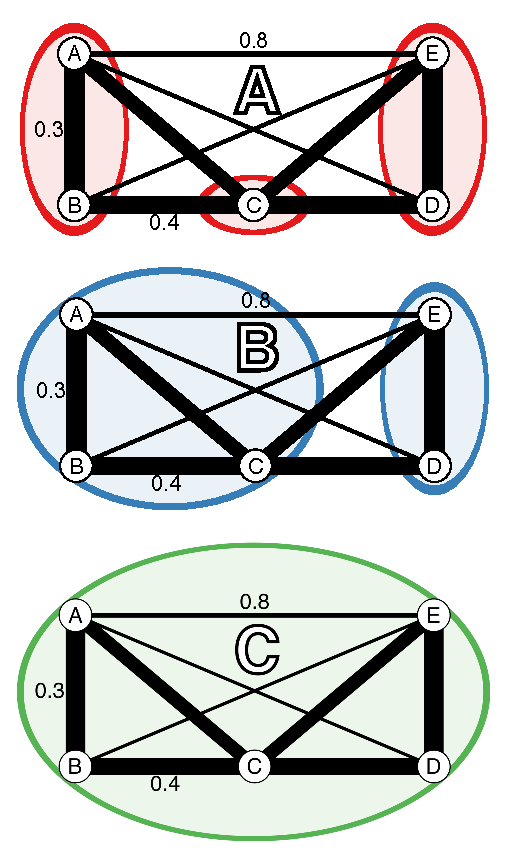
\includegraphics{poppr_frontiers_files/custom_figures/Figure-1.eps}

\subsection*{Figure 2}\label{figure-2}
\addcontentsline{toc}{subsection}{Figure 2}

\begin{CodeChunk}

\DIFdelbegin %DIFDELCMD < \includegraphics[width=85mm,height=85mm]{poppr_frontiers_files/figure-latex/Figure-2.eps} %%%
\DIFdelend \DIFaddbegin \includegraphics[width=85mm,height=85mm]{poppr_frontiers_revision_one_files/figure-latex/Figure-2-1} \DIFaddend \end{CodeChunk}

\subsection*{Figure 3}\label{figure-3}
\addcontentsline{toc}{subsection}{Figure 3}

\includegraphics{poppr_frontiers_files/custom_figures/Figure-3.eps}

\subsection*{Figure 4}\label{figure-4}
\addcontentsline{toc}{subsection}{Figure 4}

\begin{CodeChunk}

\DIFdelbegin %DIFDELCMD < \includegraphics[width=85mm,height=85mm]{poppr_frontiers_files/figure-latex/Figure-4.eps} %%%
\DIFdelend \DIFaddbegin \includegraphics[width=85mm,height=85mm]{poppr_frontiers_revision_one_files/figure-latex/Figure-4-1} \DIFaddend \end{CodeChunk}

\subsection*{Figure 5}\label{figure-5}
\addcontentsline{toc}{subsection}{Figure 5}

\begin{CodeChunk}

\DIFdelbegin %DIFDELCMD < \includegraphics[width=85mm,height=85mm]{poppr_frontiers_files/figure-latex/Figure-5.eps} %%%
\DIFdelend \DIFaddbegin \includegraphics[width=85mm,height=85mm]{poppr_frontiers_revision_one_files/figure-latex/Figure-5-1} \DIFaddend \end{CodeChunk}

\subsection*{Figure 6}\label{figure-6}
\addcontentsline{toc}{subsection}{Figure 6}

\begin{CodeChunk}

\DIFdelbegin %DIFDELCMD < \includegraphics[width=85mm,height=60mm]{poppr_frontiers_files/figure-latex/Figure-6.eps} %%%
\DIFdelend \DIFaddbegin \includegraphics[width=85mm,height=60mm]{poppr_frontiers_revision_one_files/figure-latex/Figure-6-1} \DIFaddend \end{CodeChunk}

\textbf{Table 1} Contingency table comparing multilocus lineages \DIFdelbegin \DIFdel{assigned based on average neighbor clustering (columns)
vs.~multilocus
lineages }\DIFdelend \DIFaddbegin \DIFadd{(MLL)
}\DIFaddend defined in Li et al. (2013) and Lees et al. (2006) \DIFdelbegin \DIFdel{.
}\DIFdelend \DIFaddbegin \DIFadd{(rows) to MLLs
inferred from Bruvo's genetic distance (columns) at a threshold of 0.07
with the average neighbor algorithm (Bruvo et al., 2004; Sokal, 1958).
Values in the table represent the number of times any given inferred MLL
matches with a previously defined MLL. For example, in our original data
set, there were three genotypes previously defined as the US-24 MLL. All
three genotypes were also determined to cluster into a single MLL by
filtering. In contrast, US-8 was determined to cluster into three
different MLLs by filtering.
}\DIFaddend 

\begin{table}[ht]
\centering
\DIFdelbeginFL %DIFDELCMD < \begin{tabular}{ccccccccccccccccccc}
%DIFDELCMD <   \hline
%DIFDELCMD <  %%%
\DIFdelendFL \DIFaddbeginFL \begin{tabular}{l|cccccccccccccccccc}
  \DIFaddendFL & \DIFdelbeginFL \DIFdelFL{3 }\DIFdelendFL \DIFaddbeginFL \DIFaddFL{\textbf{3} }\DIFaddendFL & \DIFdelbeginFL \DIFdelFL{4 }\DIFdelendFL \DIFaddbeginFL \DIFaddFL{\textbf{4} }\DIFaddendFL & \DIFdelbeginFL \DIFdelFL{5 }\DIFdelendFL \DIFaddbeginFL \DIFaddFL{\textbf{5} }\DIFaddendFL & \DIFdelbeginFL \DIFdelFL{6 }\DIFdelendFL \DIFaddbeginFL \DIFaddFL{\textbf{6} }\DIFaddendFL & \DIFdelbeginFL \DIFdelFL{8 }\DIFdelendFL \DIFaddbeginFL \DIFaddFL{\textbf{8} }\DIFaddendFL & \DIFdelbeginFL \DIFdelFL{10 }\DIFdelendFL \DIFaddbeginFL \DIFaddFL{\textbf{10} }\DIFaddendFL & \DIFdelbeginFL \DIFdelFL{12 }\DIFdelendFL \DIFaddbeginFL \DIFaddFL{\textbf{12} }\DIFaddendFL & \DIFdelbeginFL \DIFdelFL{15 }\DIFdelendFL \DIFaddbeginFL \DIFaddFL{\textbf{15} }\DIFaddendFL & \DIFdelbeginFL \DIFdelFL{16 }\DIFdelendFL \DIFaddbeginFL \DIFaddFL{\textbf{16} }\DIFaddendFL & \DIFdelbeginFL \DIFdelFL{17 }\DIFdelendFL \DIFaddbeginFL \DIFaddFL{\textbf{17} }\DIFaddendFL & \DIFdelbeginFL \DIFdelFL{18 }\DIFdelendFL \DIFaddbeginFL \DIFaddFL{\textbf{18} }\DIFaddendFL & \DIFdelbeginFL \DIFdelFL{20 }\DIFdelendFL \DIFaddbeginFL \DIFaddFL{\textbf{20} }\DIFaddendFL & \DIFdelbeginFL \DIFdelFL{21 }\DIFdelendFL \DIFaddbeginFL \DIFaddFL{\textbf{21} }\DIFaddendFL & \DIFdelbeginFL \DIFdelFL{22 }\DIFdelendFL \DIFaddbeginFL \DIFaddFL{\textbf{22} }\DIFaddendFL & \DIFdelbeginFL \DIFdelFL{24 }\DIFdelendFL \DIFaddbeginFL \DIFaddFL{\textbf{24} }\DIFaddendFL & \DIFdelbeginFL \DIFdelFL{25 }\DIFdelendFL \DIFaddbeginFL \DIFaddFL{\textbf{25} }\DIFaddendFL & \DIFdelbeginFL \DIFdelFL{27 }\DIFdelendFL \DIFaddbeginFL \DIFaddFL{\textbf{27} }\DIFaddendFL & \DIFdelbeginFL \DIFdelFL{28 }\DIFdelendFL \DIFaddbeginFL \DIFaddFL{\textbf{28} }\DIFaddendFL \\ 
  \hline
\DIFdelbeginFL \DIFdelFL{B }\DIFdelendFL \DIFaddbeginFL \DIFaddFL{\textbf{B} }\DIFaddendFL & . & . & . & . & . & . & . & . & . & . & . & . & . & . & . & 1 & . & . \\ 
  \DIFdelbeginFL \DIFdelFL{C }\DIFdelendFL \DIFaddbeginFL \DIFaddFL{\textbf{C} }\DIFaddendFL & . & . & . & . & . & . & . & . & . & . & . & . & . & . & 1 & . & . & . \\ 
  \DIFdelbeginFL \DIFdelFL{D.1 }\DIFdelendFL \DIFaddbeginFL \DIFaddFL{\textbf{D.1} }\DIFaddendFL & . & . & . & . & . & . & . & . & . & . & . & . & . & 1 & . & . & . & . \\ 
  \DIFdelbeginFL \DIFdelFL{D.2 }\DIFdelendFL \DIFaddbeginFL \DIFaddFL{\textbf{D.2} }\DIFaddendFL & . & . & . & . & . & . & . & . & . & . & . & . & . & 1 & . & . & . & . \\ 
  \DIFdelbeginFL \DIFdelFL{EU-13 }\DIFdelendFL \DIFaddbeginFL \DIFaddFL{\textbf{EU-13} }\DIFaddendFL & . & . & . & . & . & . & . & . & 1 & . & . & . & . & . & . & . & . & . \\ 
  \DIFdelbeginFL \DIFdelFL{EU-4 }\DIFdelendFL \DIFaddbeginFL \DIFaddFL{\textbf{EU-4} }\DIFaddendFL & . & . & . & . & . & . & . & . & . & 1 & . & . & . & . & . & . & . & . \\ 
  \DIFdelbeginFL \DIFdelFL{EU-5 }\DIFdelendFL \DIFaddbeginFL \DIFaddFL{\textbf{EU-5} }\DIFaddendFL & . & . & . & . & . & . & . & . & . & . & 2 & . & . & . & . & . & . & . \\ 
  \DIFdelbeginFL \DIFdelFL{EU-8 }\DIFdelendFL \DIFaddbeginFL \DIFaddFL{\textbf{EU-8} }\DIFaddendFL & . & . & . & . & . & . & 1 & . & . & . & . & . & . & . & . & . & . & . \\ 
  \DIFdelbeginFL \DIFdelFL{US-11 }\DIFdelendFL \DIFaddbeginFL \DIFaddFL{\textbf{US-11} }\DIFaddendFL & . & . & . & . & . & . & . & . & . & . & . & . & . & . & . & . & . & 2 \\ 
  \DIFdelbeginFL \DIFdelFL{US-12 }\DIFdelendFL \DIFaddbeginFL \DIFaddFL{\textbf{US-12} }\DIFaddendFL & . & 1 & . & . & . & . & . & . & . & . & . & . & . & . & . & . & . & . \\ 
  \DIFdelbeginFL \DIFdelFL{US-14 }\DIFdelendFL \DIFaddbeginFL \DIFaddFL{\textbf{US-14} }\DIFaddendFL & . & . & . & . & . & 1 & . & . & . & . & . & . & . & . & . & . & . & . \\ 
  \DIFdelbeginFL \DIFdelFL{US-17 }\DIFdelendFL \DIFaddbeginFL \DIFaddFL{\textbf{US-17} }\DIFaddendFL & . & . & . & . & . & . & . & . & . & . & . & 1 & . & . & . & . & . & . \\ 
  \DIFdelbeginFL \DIFdelFL{US-20 }\DIFdelendFL \DIFaddbeginFL \DIFaddFL{\textbf{US-20} }\DIFaddendFL & 2 & . & . & . & . & . & . & . & . & . & . & . & . & . & . & . & . & . \\ 
  \DIFdelbeginFL \DIFdelFL{US-21 }\DIFdelendFL \DIFaddbeginFL \DIFaddFL{\textbf{US-21} }\DIFaddendFL & . & . & . & . & . & . & . & . & . & . & . & . & . & . & . & . & 2 & . \\ 
  \DIFdelbeginFL \DIFdelFL{US-22 }\DIFdelendFL \DIFaddbeginFL \DIFaddFL{\textbf{US-22} }\DIFaddendFL & . & . & . & . & . & . & . & . & . & . & . & . & 2 & . & . & . & . & . \\ 
  \DIFdelbeginFL \DIFdelFL{US-23 }\DIFdelendFL \DIFaddbeginFL \DIFaddFL{\textbf{US-23} }\DIFaddendFL & . & . & . & . & . & . & . & 3 & . & . & . & . & . & . & . & . & . & . \\ 
  \DIFdelbeginFL \DIFdelFL{US-24 }\DIFdelendFL \DIFaddbeginFL \DIFaddFL{\textbf{US-24} }\DIFaddendFL & . & . & . & . & 3 & . & . & . & . & . & . & . & . & . & . & . & . & . \\ 
  \DIFdelbeginFL \DIFdelFL{US-8 }\DIFdelendFL \DIFaddbeginFL \DIFaddFL{\textbf{US-8} }\DIFaddendFL & . & . & 1 & 1 & . & 2 & . & . & . & . & . & . & . & . & . & . & . & . \\ 
   \hline
\end{tabular}
\end{table}

\section*{Figure Legends}\label{figure-legends}
\addcontentsline{toc}{section}{Figure Legends}

\textbf{Figure 1} Diagrammatic representation of the three clustering
algorithms implemented in \texttt{mlg.filter}. (\textbf{A-C}) Represent
different clustering algorithms on the same imaginary network with a
threshold of 0.451. Edge weights are represented in arbitrary units
noted by the line thickness and numerical values next to the lines. All
outer angles are 90 degrees, so the un-labeled edge weights can be
obtained with simply geometry. Colored circles represent clusters of
genotypes. (\textbf{A}) Farthest neighbor clustering does not cluster
nodes B and C because nodes A and C are more than a distance of 0.451
apart. (\textbf{B}) UPGMA (average neighbor) clustering clusters nodes
A, B, and C together because the average distance between them and C is
\textless{} 0.451. (\textbf{C}) Nearest neighbor clustering clusters all
nodes together because the minimum distance between them is always
\textless{} 0.451.

\textbf{Figure 2} Graphical representation of three different clustering
algorithms collapsing multilocus genotypes for 12 SSR loci from
\emph{Phytophthora infestans} representing 18 clonal lineages. The
horizontal axis is Bruvo's genetic distance assuming the genome addition
model. The vertical axis represents the number of multilocus lineages
observed. Each point shows the threshold at which one would observe a
given number of multilocus genotypes. The horizontal black line
represents 18 multilocus genotypes and vertical dashed lines mark the
thresholds used to collapse the multilocus genotypes into 18 multilocus
lineages.

\textbf{Figure 3} (\textbf{A-B}) Minimum spanning networks of the
hemagglutinin (HA) segment of H3N2 viral DNA from the \emph{adegenet}
package representing flu epidemics from 2001 to 2006 without
reticulation (\textbf{A}) and with reticulation (\textbf{B}) (Jombart,
2008; Jombart et al., 2010). Each node represents a unique multilocus
genotype, colors represent epidemic year, and edge color represents
absolute genetic distance. (\textbf{C}) Shannon entropy values for
population assignments compared with communities determined by the
infoMAP algorithm on (\textbf{A}) and (\textbf{B}). (\textbf{D}) Graphic
reproduced from Jombart et al. (2010) showing that the 2006 epidemic
does not cluster neatly with the other years \DIFaddbegin \DIFadd{via Discriminant Analysis
of Principal Components. Horizontal axis represents the first
discriminant component. Vertical axis represents the second discriminant
component}\DIFaddend .

\textbf{Figure 4} UPGMA dendrogram generated from Nei's genetic distance
on 15 breeds of \emph{Bos taurus} (BT) or \emph{Bos indicus} (BI) from
Africa (AF) or France (FR). These data are from Lalo{\"{e}} et al. (2007).
Node labels represent bootstrap support \(>50\%\) out of 1,000 bootstrap
replicates.

\textbf{Figure 5} Genotype accumulation curve for 694 isolates of the
peach brown rot pathogen, \emph{Monilinia fructicola} genotyped over 13
loci from Everhart and Scherm (2015). The horizontal axis represents the
number of loci randomly sampled without replacement up to \(n - 1\)
loci, the vertical axis shows the number of multilocus genotypes
observed, up to 262, the number of unique multilocus genotypes in the
data set. The red dashed line represents 90\% of the total observed
multilocus genotypes. A trendline (blue) has been added using the
\emph{ggplot2} function \texttt{stat\_smooth}.

\textbf{Figure 6} \textbf{(A)} Sliding window analysis of the
standardized index of association (\(\bar{r}_d\)) across a simulated
\(1.1 \times 10^4\) nt chromosome containing 1,100 variants among 100
individuals. Each window analyzed variants within 500nt chunks. The
black line refers to the clonal and the blue line to the sexual
populations. \textbf{(B)} boxplots showing 100 random samples of 50
variants to calculate a distribution of \(\bar{r}_d\) for the clonal
(red) and sexual (blue) populations. Each box is centered around the
mean, with whiskers extending out to 1.5 times the interquartile range.
The median is indicated by the center line. \textbf{(A)} and
\textbf{(B)} are plotted on the same y-axis.

\end{document}

